
\subsubsection{Overview}

The Referee Box (Refbox) is an external component build by Aachen University. This component controls, monitors, and evaluates the game during the Robocup. It communicates with robots of both teams and the MPS, attributes the points and manages the different phases of the game. To get more information, it is recommended to read the referee box manual located at \url{http://www.robocup-logistics.org/refbox}. To set up the Refbox, the file “config.yaml” should be modified. The most important part to change in this file is the IP addresses (cf. Figure \ref{fig:configFile1}). \\

\begin{figure}[!h]
\centering
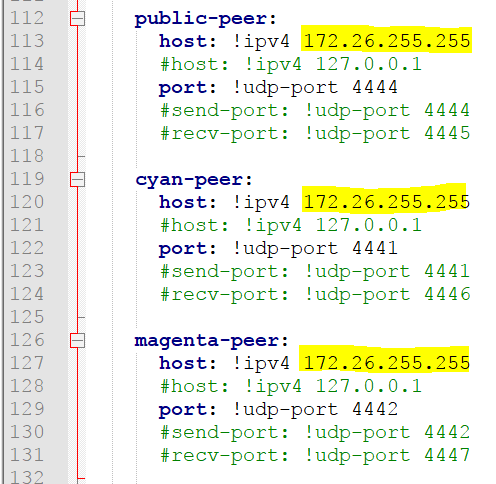
\includegraphics[]{pic/config_file_1.png}
\caption{IP adresses to modify in the config.yaml file}
\label{fig:configFile1}
\end{figure}

It is also needed to define a name for the team and a crypto key. It should be the same key in the Refbox server component.

\begin{figure}[!h]
\centering
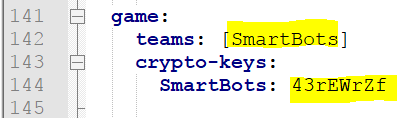
\includegraphics[]{pic/config_file_2.png}
\caption{Name and key to modify in config file}
\label{fig:configFile2}
\end{figure}

To run the Refbox, two programs should be executed at the same time: the main program (llsf-refbox) and the graphical interface (llsf-refbox-shell).

\begin{figure}[!h]
\centering
\includegraphics[width=\linewidth]{pic/graphical_refbox.png}
\caption{Graphical interface of the Refbox during Robocup 2017}
\label{fig:graphicalRefbox}
\end{figure}

\subsubsection{Situation in 2016}

There was no permanent Refbox installed in the laboratory. Each team was forced to install the Refbox software with all necessary libraries on a workstation or on his own computer. \\

\subsubsection{Situation in 2017}

During this year, a permanent Refbox with all the necessary libraries for the Robocup 2017 version (Branch tneumann/rcll17 in the git repository) has been installed on an independent laptop. Any person that needs to test situations with the Refbox can easily take the laptop near his computer or access the laptop via XTightVncViewer. To do this, it is necessary to run the VNC server on the laptop with the command “tightvncserver”. Then it is possible to access with the command “xtightvncviewer <<ipAdress>> :1”.  In the current network, the IP address is bounded to “172.26.1.112”. A window will be open and an access to the Refbox is possible (cf. Figure \ref{fig:xtightvncviewer}).\\

\begin{figure}[!h]
\centering
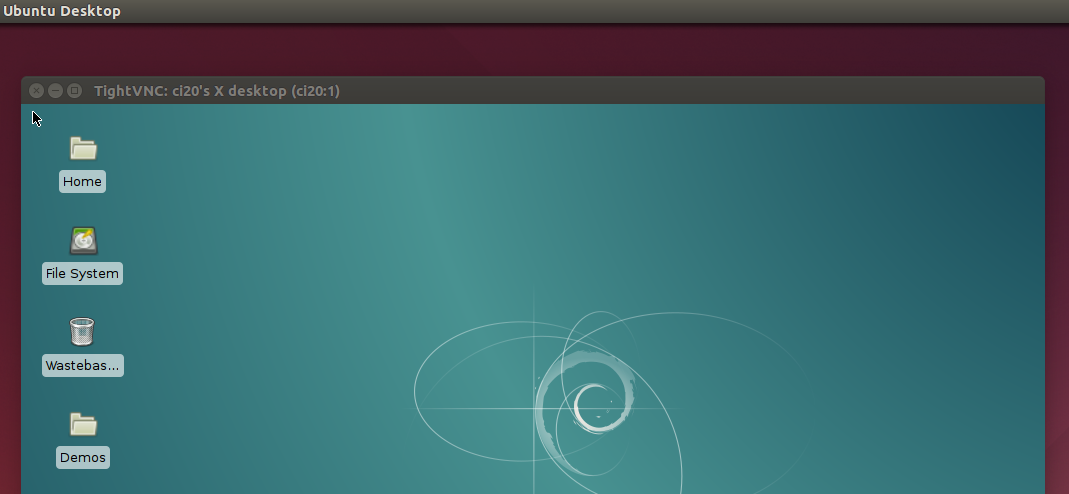
\includegraphics[width=\linewidth]{pic/xtightvncviewer.png}
\caption{Remote access to the Refbox laptop with XTightVncViewer}
\label{fig:xtightvncviewer}
\end{figure}

The Refbox software is constantly developed further so it is necessary to update the local Refbox in the lab to the lastest version. All versions can be found in this repository: \url{https://git.fawkesrobotics.org/llsf-refbox.git}. A contact with Tim Niemueller \cite{RC2017}, one of the main developers of the Refbox, should be established to have information about the version used at the competition. \\


\subsubsection{Difficulties}

During the Robocup 2017, some difficulties have been faced. First, it is not possible for the team to pre-assign zones where MPS stations are located. This means that testing in the lab is quite hard because only a small part of the field can be mapped to the zafh-lab. Because of this problem it was only tested if the Refbox can detect the MPS report from the Robotinos. It was not tested whether the correct MPS was detected but only if a MPS was detected by the Refbox. Another problem was to get the latest version of the Refbox. At the time of the Robocup the last version of the repository trunk was used in the Robocup 2016. It was required to search through the git repository to find the correct version of the Refbox. This version can be found on the tneumann/rcll17 branch. The last point was that the network setup was not easy during the Robocup. Therefore the team should have a Refbox for testing which has the same setup than the offical Refbox used in the competition. \\
